% To ponder: What is the goal of this paper? What would I want to know if I was reading it? What is the narrative? What makes this important research?
\section{Introduction}
% Motivation
% Pronunciation is crucial in the acquisition of a second language (L2). While pronunciation can gradually improve during acquisition through implicit immersion, explicit pronunciation practice improves it at a faster rate~\cite{carey_call_2004,hew_effect_2004,offerman_visual_2016,yuen_enunciate_2011,sherwin_natural_2018,skalski_mapping_2011,vanden2013more}. Learners who practice pronunciation with visual feedback outperform their peers who used other methods of practice~\cite{carey_call_2004,hew_effect_2004,offerman_visual_2016,yuen_enunciate_2011}. Many visual feedback systems have a steep learning curve to understand and act on the feedback. 
% While many studies interview learners about their experience post interaction with a tool, there is lack of understanding of how interactions with visual versus audio-only feedback affects learners awareness of their pronunciation as a whole. 


% why is learning pronunciation in a second language is hard
Every speaker comes with their own language background and physical characteristics, thus, pronunciation feedback must be personalized for second language learners. Individualizing feedback requires more time from language teachers in a system already strained by the lack of instructors~\cite{moser2024covid,hismanoglu2010language,rao2019key,munro2015setting}. Computer-Assisted Pronunciation Training (CAPT) has the potential to assist learners by providing feedback specific to their needs. Although CAPT introduces the potential for algorithmic error and requires access to computing resources, it addresses the drawbacks of a teacher-dependent model. It does not require extra time from a teacher, is widely distributable, and provides access to practice in a self-paced environment. Among CAPT methods, visual feedback has arisen as an effective way to provide pronunciation feedback~\cite{carey_call_2004,hew_effect_2004,offerman_visual_2016,yuen_enunciate_2011}.   

% why do we need to study visual feedback methods? What has been done? What is lacking?
There are two main types of visual feedback for pronunciation: correctness indicators, such as color coding or percentages, and articulation-based representation of speech. Many well-known language learning apps, such as Duolingo, babbel, and Rosetta Stone, use correctness-based visual feedback, while previous research focuses on articulation-based visualizations (ABV)~\cite{carey_call_2004,hew_effect_2004,offerman_visual_2016}. We choose an ABV because it satisfies all the criteria in Bliss et. al.~\cite{bliss2018computer} for effective feedback. Correctness-based feedback fails two of the criteria; namely, feedback must be (i) natural and logical and (ii) able to facilitate comparison~\cite{bliss2018computer}. Since color coding and percentages do not specify what about the production is incorrect, correctness-based feedback fails to be natural and logical. It fails the latter by forcing learners to use their ears to determine the differences instead of visually representing comparisons. 

% , such as simple color coded levels of correct and incorrect,
% 
\begin{figure*}[t]
    \centering
    \begin{tabular}{c c}  % Two-column image layout
        \begin{subfigure}{0.45\textwidth}
            \centering
            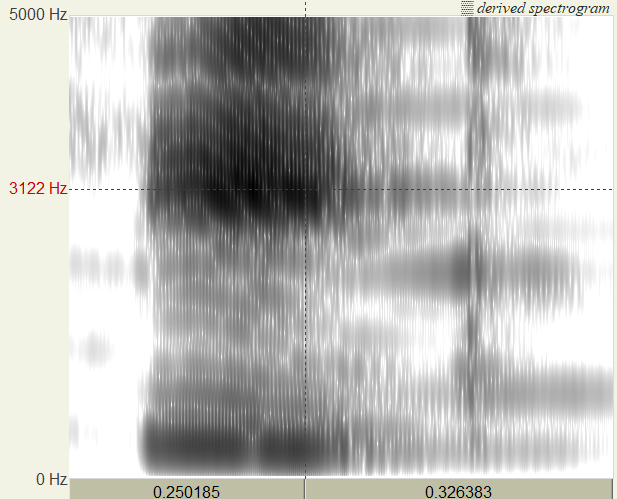
\includegraphics[width=\linewidth]{pictures/intro/praat_spectrogram.png}
            \caption{A spectrogram from Praat of the English word "Heat".}
            \label{fig:specHeat}
        \end{subfigure} &
        \begin{subfigure}{0.45\textwidth}
            \centering
            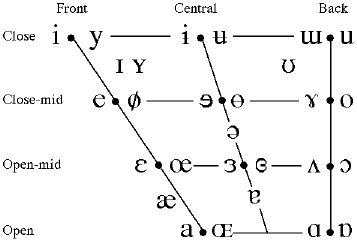
\includegraphics[width=\linewidth]{pictures/intro/vowel-chart-of-the-International-Phonetic-Alphabet.png}
            \caption{An example vowel chart~\cite{wieling2011inducing}.  The x-axis represents the second formant and frontedness or backedness of the tongue. The y-axis is the first formant and height of the tongue in the mouth.}
             \label{fig:exampleVwlChart}
        \end{subfigure} \\

        \begin{subfigure}{0.45\textwidth}
            \centering
            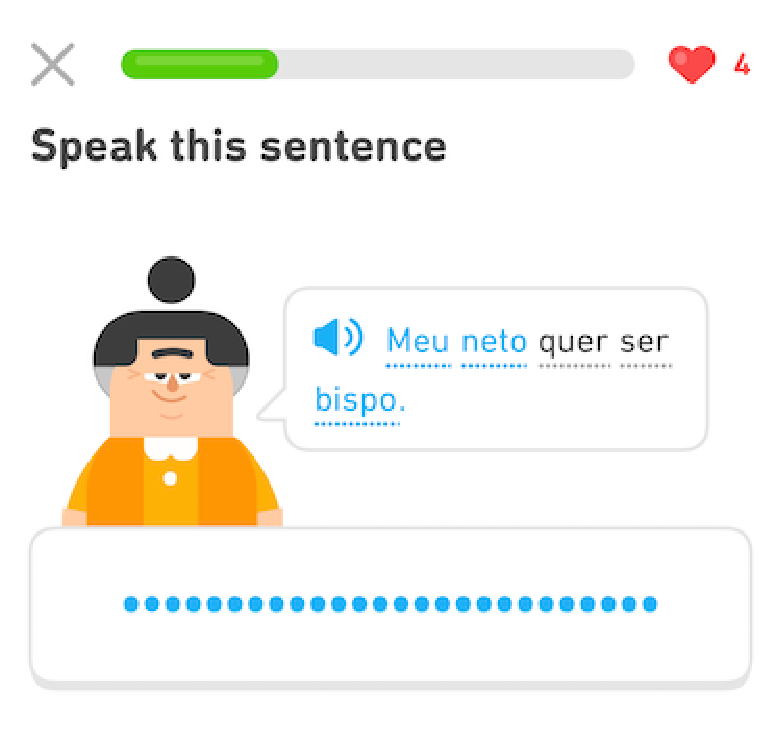
\includegraphics[width=\linewidth]{pictures/intro/Speaking_3_CharacterSpeakBlue.pdf}
        \caption{A screenshot of Duolingo's binary speaking feedback as of 2020~\cite{Blanco_Moline_2025}}.
        \label{fig:VOTexample}
        \end{subfigure} &
        \begin{subfigure}{0.45\textwidth}
            \centering
            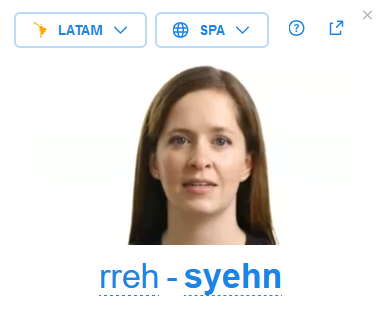
\includegraphics[width=\linewidth]{pictures/intro/spaDict_face.png}
        \caption{A still frame from a video of a speaker's face on SpanishDict.com.}
        \label{fig:facialFeature}
        \end{subfigure}
    \end{tabular}

    % \vspace{10pt} % Adjust spacing before the caption

    \caption{Four types of pronunciation visualizations.}
    \label{fig:proVisualizationEx}
\end{figure*}
Three widely studied visual feedback methods are the spectrogram, animated face-cutaways, and the vowel chart. The spectrogram, which can be used for both vowels and consonants, is difficult to interpret without training and hard to modify pronunciation based on its feedback (Figure~\ref{fig:specHeat}). Animated face-cutaways and vowel charts, which provide feedback on a subset of sounds, have fewer parts to interpret and uses the principle of natural mapping to visualizes articulator movement (Figure~\ref{fig:exampleVwlChart}). The vowel chart follows more closely the principles of effective feedback and is effective in improving pronunciation~\cite{rehman2021real,carey_call_2004}. Previous implementation of vowel charts, however, do not fully integrate audio and visual. Users had to adjust pronunciation based either on visual or audio output. For this reason, we created an interactive version, \visowel{}. The chart displays the position of the tongue based on the first and second formants, prominent bands of energy based around a frequency~\cite{schaferFormant1970}. \visowel{} provides broad applicability by accepting vowels within multiple contexts including rhotics, like the American /r/\footnote{The forward slash (/) represents the orthographic character in a language. Square brackets around a character indicate a phonetic description.} and displays a vowel's change over time, allowing learners to train the difference between single vowels (monophthongs) and combined vowels (diphthongs). As far as we are aware, we are the first study to have vowels in multiple contexts, visuals for diphthongs, and \textbf{the first study in visual Computer-Assisted Pronunciation Training (CAPT) to capture how learners interpret visual results as they adjust their pronunciation}.

%A spectrogram visualizes the amplitudes of frequencies in a sound signal. A vowel chart uses the principle of natural mapping which has been applied in many domains with positive results to map the position of the tongue to a position on the chart~\cite{sherwin_natural_2018,skalski_mapping_2011,vanden2013more}.
%obile interface design, physical automobile controls, and video game controller design with positive results. 

% Research Questions

Using an iterative design approach, we created \visowel{} and an audio-only practice tool. We ran a within-subject study with 8 participants and elicited speakers' real-time thought processes as they used both tools. 

\visowel{} encouraged participants to practice more because it gave them a goal to work toward or pushed them to reflect on the first language speaker's production and their own when visual results did not align with their expectations. Based on our findings, we suggest that future pronunciation feedback should include a visual representation of the closeness of the learner and target speaker.

Our work makes three main contributions.
\begin{enumerate}
    \item Learners' thought processes during interaction with visual pronunciation feedback.
    \item An interactive vowel chart, \visowel{}, that can be used in any word context.
    \item A technical implementation for extracting vowels from any context.
\end{enumerate}


